% Autor: Leonhard Segger, Alexander Neuwirth
% Datum: 2017-10-30
\documentclass[
	% Papierformat
	a4paper,
	% Schriftgröße (beliebige Größen mit „fontsize=Xpt“)
	12pt,
	% Schreibt die Papiergröße korrekt ins Ausgabedokument
	pagesize,
	% Sprache für z.B. Babel
	ngerman
]{scrartcl}

% Achtung: Die Reihenfolge der Pakete kann (leider) wichtig sein!
% Insbesondere sollten (so wie hier) babel, fontenc und inputenc (in dieser
% Reihenfolge) als Erstes und hyperref und cleveref (Reihenfolge auch hier
% beachten) als Letztes geladen werden!

% Silbentrennung etc.; Sprache wird durch Option bei \documentclass festgelegt
\usepackage{babel}
% Verwendung der Zeichentabelle T1 (Sonderzeichen etc.)
\usepackage[T1]{fontenc}
% Legt die Zeichenkodierung der Eingabedatei fest, z.B. UTF-8
\usepackage[utf8]{inputenc}
% Schriftart
\usepackage{lmodern}
% Zusätzliche Sonderzeichen
\usepackage{textcomp}

% Mathepaket (intlimits: Grenzen über/unter Integralzeichen)
\usepackage[intlimits]{amsmath}
% Ermöglicht die Nutzung von \SI{Zahl}{Einheit} u.a.
\usepackage{siunitx}
% Zum flexiblen Einbinden von Grafiken (\includegraphics)
\usepackage{graphicx}
% Abbildungen im Fließtext
\usepackage{wrapfig}
% Abbildungen nebeneinander (subfigure, subtable)
\usepackage{subcaption}
% Funktionen für Anführungszeichen
\usepackage{csquotes}
% Zitieren, Bibliographie
\usepackage{biblatex}

% Verlinkt Textstellen im PDF-Dokument
\usepackage[unicode]{hyperref}
% "Schlaue" Referenzen (nach hyperref laden!)
\usepackage{cleveref}
% Zur Darstellung von Webadressen
\usepackage{url}
%chemische Formeln
\usepackage[version=4]{mhchem}
% siunitx: Deutsche Ausgabe, Messfehler getrennt mit ± ausgeben
\usepackage{floatrow}
\floatsetup[table]{capposition=top}
\sisetup{
	locale=DE,
	separate-uncertainty
}
%\bibliography{6Mi_S2_25-10-2017_References}

\begin{document}
	
	\begin{titlepage}
		\centering
		{\scshape\LARGE Versuchsbericht zu \par}
		\vspace{1cm}
		{\scshape\huge M1 - Drehpendel nach Pohl\par}
		\vspace{2.5cm}
		{\LARGE Gruppe 6Mi \par}
		\vspace{0.5cm}
		
		{\large Alexander Neuwirth (E-Mail: a\_neuw01@wwu.de) \par}
		{\large Leonhard Segger (E-Mail: l\_segg03@uni-muenster.de) \par}
		\vfill
		
		durchgeführt am 21.11.2017\par
		betreut von\par
		{\large Torsten Stiehm}
		
		\vfill
		
		{\large \today\par}
	\end{titlepage}
	\tableofcontents
	\newpage
	
	\section{Kurzfassung}
	Das Drehpendel nach Pohl ist ein Beispiel für schwingfähige Systeme.
	\section{Methoden}
	
	\subsection{Drehpendel ohne Dämpfung}%...
	Zunächst haben wir die Eigenfrequenz, bzw. Periodendauer, des Drehpendels (annähernd) ohne Dämpfung mithilfe einer Stoppuhr bestimmt. Um den Fehler, der durch die menschliche Reaktionszeit entsteht, zu minimieren, haben wir die Zeit, die das Drehpendel für 20 Schwingungen benötigt, gemessen, um dann über diese zu mitteln.
	Als Anfangs- und Endpunkt der Messung haben wir die Ruhelage der Scheibe gewählt, da sie sich dort näherungsweise mit konstanter Geschwindigkeit bewegt und man somit den Reaktionsfehler leichter ausgleichen kann.
	Alternativ hätte man den linken oder rechten Wendepunkt der Bewegung wählen können. An dieser Stelle bewegt sich das Pendel allerdings langsam und der Zeitraum, in dem das Pendel stillsteht, ist verhältnismässig groß, weshalb das Ende der Bewegung kaum exakt zu erkennen ist. %Von sich selbst darf man ja wohl plagiarisieren.
	Dann haben wir dieselbe Messung erneut durchgeführt. Diesmal wurde die Drehung digital mit einem Messrad, welches durch einem Faden mit dem Schwingrad verbunden war, erfasst und als Messkurve mit dem Computer aufgezeichnet.%Cyber Cyber
	\subsection{Drehpendel mit Dämpfung}
	Im Anschluss daran fügten wir eine Dämpfung in Form einer Wirbelstrombremse hinzu. Von dem sich ergebenden Schwingungsvorgang haben wir drei Messkurven mit jeweils unterschiedlichen Dämpfungen, also unterschiedlichem Stromfluss durch die Spulen der Wirbelstrombremse, aufgenommen. Hieraus konnten wir jeweils die Eigenfrequenz und die Dämpfung aus der Abnahme der Amplitude bestimmen. %Sollte man hier die konkreten Werte des Stromflusses nennen? Denke nicht.
	\subsection{Drehpendel mit Exzenter und Dämpfung} 
	Nun haben wir das Drehpendel mit einem Exzenter (in Form eines Motors, der die Spiralfeder anregt) und der Wirbelstrombremse betrieben. Hierbei haben wir darauf geachtet die Messung erst zu starten, nachdem das Pendel die Einschwingphase überwunden hatte, also sich Frequenz und Amplitude nicht mehr merklich änderten.
	Zunächst nahmen wir eine Kalibrierkurve auf, um den Zusammenhang zwischen der Frequenz der Anregung $\omega$ und der Spannung am Tacho-Ausgang des Motors zu quantifizieren.
	Anschließend haben wir für drei verschiedene Dämpfungen je 20 Messungen mit unterschiedlicher Anregungsfrequenz $\omega$ durchgeführt. Gemessen wurde jeweils für ca. \SI{20}{\second}. 
	\subsection{Qualitative Beobachtungen und Vergleich zum Fadenpendel}
	Wir haben bei kleiner Dämpfung den Phasenunterschied zwischen Anregung und Drehpendel bei Frequenzen über, unter und nahe bei der Resonanzfrequenz beobachtet. Dann haben wir dieselbe Untersuchung bei einem Fadenpendel durchgeführt, um die Parallelen erkennen zu können.
	\subsection{Einführung einer Nichtlinearität}
	Zuletzt wurde noch eine Nichtlinearität in Form eines kleinen Gewichtes eingeführt. Diese Gewicht haben wir am oberen Rand der Scheibe (eine Daumenbreite neben dem obersten Punkt) in Ruhelage befestigt. Dann haben wir das Verhalten des Drehpendels bei steigender sowie bei sinkender Anregungsfrequenz beobachtet. Anschließend haben wir näherungsweise die Resonanzfrequenz eingestellt und die Schwingung beobachtet.
	
	\section{Ergebnisse und Diskussion}
	
	\subsection{Drehpendel ohne Dämpfung}
	Die Messung mit einer Stoppuhr ergibt eine Dauer von $T_{20} =\SI{28,15}{\second}$ für 20 Schwingungen, also pro Schwingung $ T_\text{Uhr} = \SI{1,41}{\second}$. %TODO seltsame Underfull hbox Warnung
	Für die Unsicherheit von \(T\) gilt: \\
	\begin{itemize}
		\item  Digitalanzeige der Stoppuhr \SI{\pm 0,005}{\second}, (Typ B): \( u_B(T) = \frac{2\cdot \SI{0,005}{\second}}{2 \cdot 20 \sqrt{3}} = \SI{0,00014}{\second} \)
		\item Reaktionszeit \SI{\pm 0,1}{\second}, (Typ B): \( u_B(T) \approx \frac{2\cdot \SI{0,1}{\second}}{2 \cdot 20 \sqrt{3}} = 0.0029\si{s} \)
		\item Komb. Unsicherheit: $ u_\text{Uhr}(T) = \sqrt{(0,00014\si{s})^2+(0.0029\si{s})^2} \approx 0,0029 \si{s} $
	\end{itemize} 
	$ \implies T_\text{Uhr} = \SI{1,41 \pm 0,0029}{\second} $ \newline 
	Für die Frequenz ergibt sich daraus $ f_\text{Uhr} = \frac{1}{T_\text{Uhr}} = \SI{0,71}{\per \second}$ und für die Unsicherheit: \newline
	
	\begin{equation*}
		u_\text{Uhr}(f) = \left|  \frac{\partial f}{\partial T_\text{Uhr}} u_\text{Uhr}(T_\text{Uhr}) \right| = \left| - \frac{1}{T_\text{Uhr}^2}u_\text{Uhr}(T_\text{Uhr}) \right| \approx \SI{0,0015}{\per \second} %Ich hoffe mal das ist rechnerisch richtig, man könnte sich beschweren, dass wir bei der Unsicherheit mehr Stellen von f,t,u angeben müssten
	\end{equation*}
	Insgesamt: $f_\text{Uhr} = \SI{0,709 \pm 0,0015}{\per \second}  $ \\
	\begin{figure}[htb]
		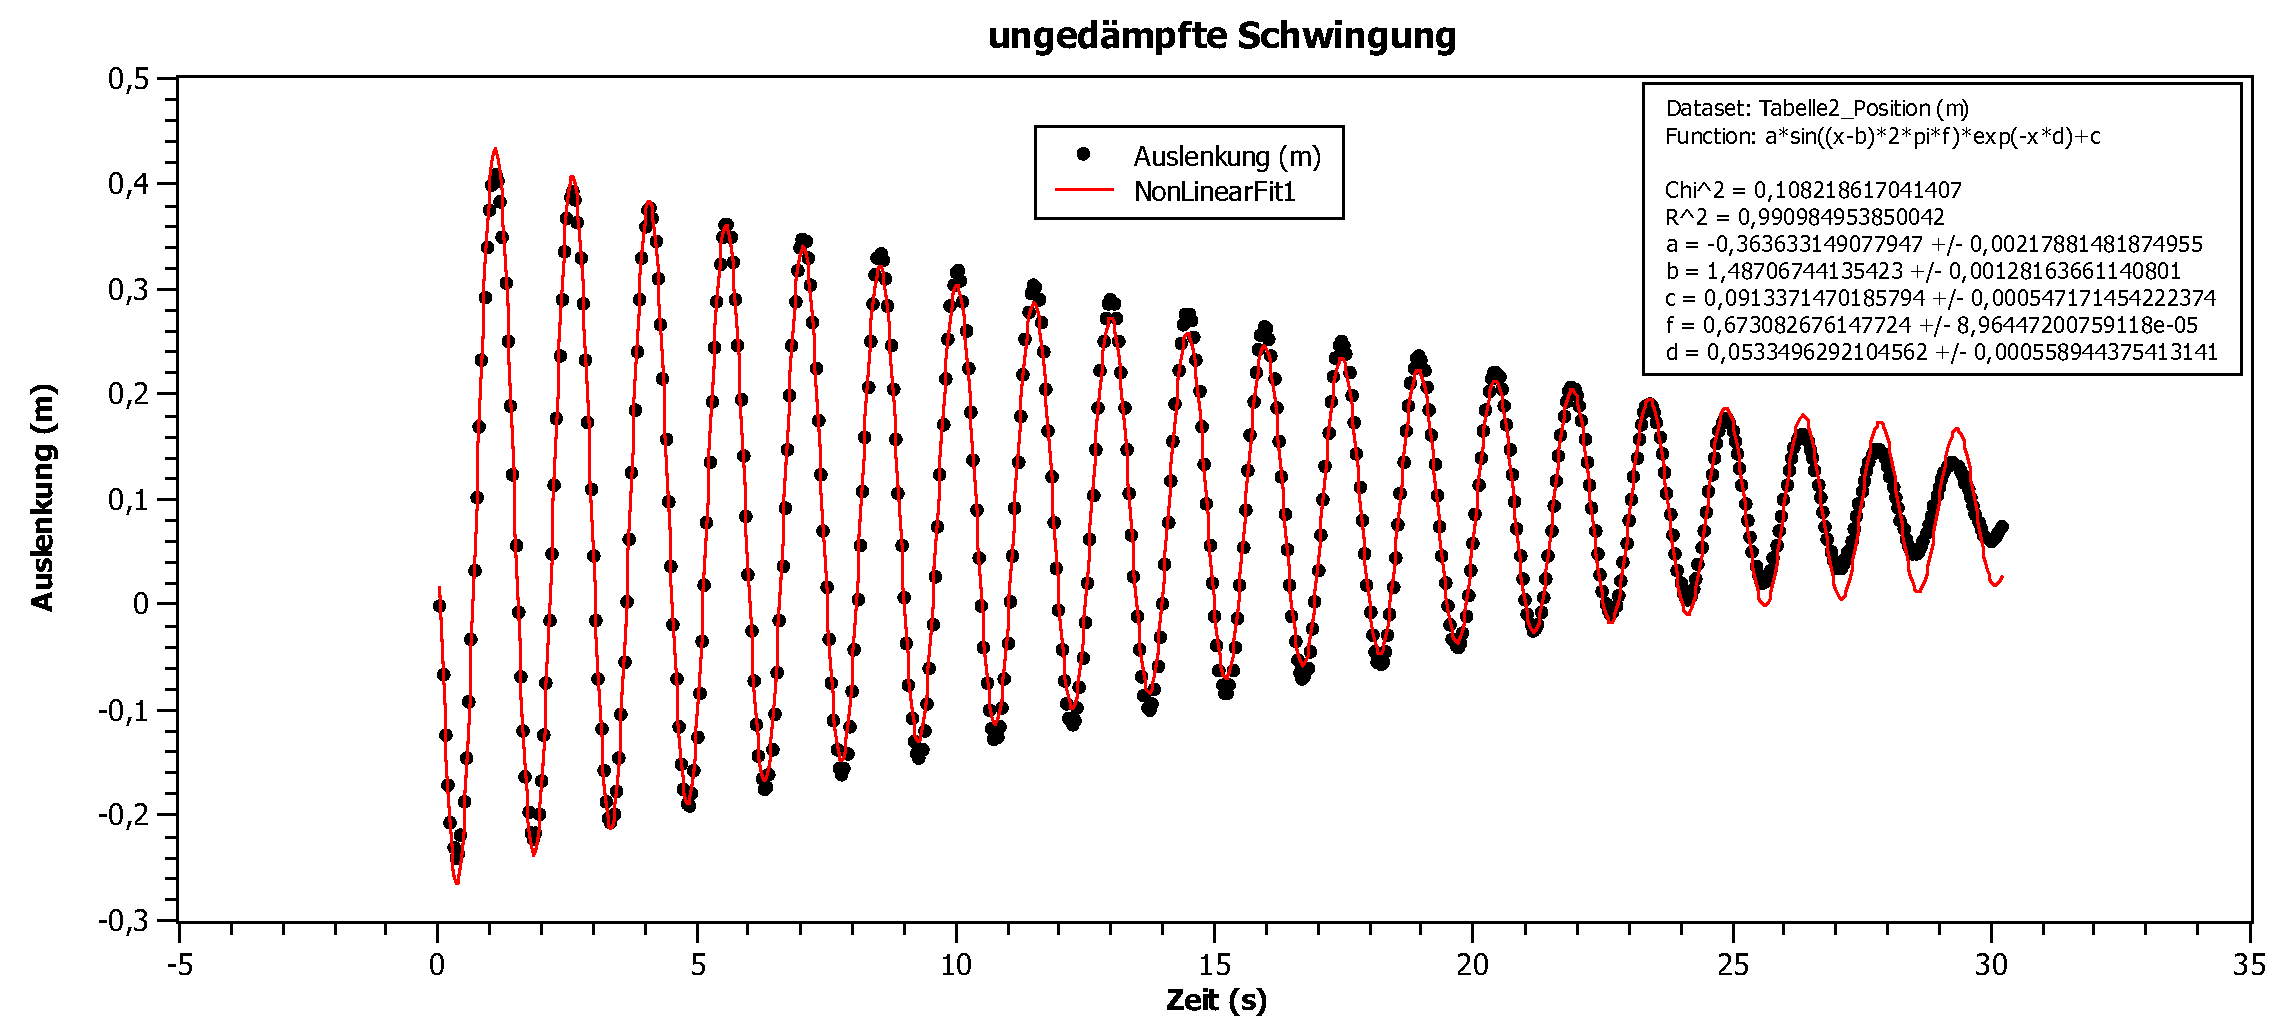
\includegraphics[width=1\textwidth]{Ungedaempfte_Schwingung_Graph}
		\centering
		\caption{Das Ergebnis der mit dem Computer aufgezeichneten Messkurve für die ungedämpfte Schwingung}
		\label{ungedämpfte_Schwingung}
		\centering
	\end{figure}
	In \cref{ungedämpfte_Schwingung} wurden die Messergebnisse der (näherungsweise) ungedämpften Schwingung aufgetragen. Dann wurde ein Fit gemäß dem \enquote{Scaled Levenberg-Marquardt algorithm} mit der zugrunde liegenden Funktion
	\begin{equation}
	y(t) = a \sin ((x-b)2 \pi f) \exp^{-x \cdot b} + c
	\end{equation}
	
	durchgeführt. Dabei ist $a$ die Amplitude bei $t=0$, $b$ die Phase bei $t=0$  (beides nicht weiter interessant, weil nur abhängig vom Beginn der Messung), $f$ die Frequenz und $d$ die Dämpfung.\\
	Zusätzlich entsteht eine Unsicherheit durch ein mögliches Mitrutschen des Seils an beiden Scheiben, den wir im Folgenden großzügig mit 
	\begin{equation*}
		u(y) = \frac{2 \cdot \SI{0,01}{\meter}}{2 \sqrt{3}} \approx \SI{0,0058}{\meter}
	\end{equation*}
	abschätzen. Da die Bewegung allerdings gleichermaßen in beide Richtungen stattfindet, wird dieser Fehler nicht mit steigender Messungsdauer größer.
	Wir gehen davon aus, dass der unbekannte Fehler des Messgerätes in Bezug auf die Auslenkung gegenüber jenem verschwindet. Gleiches nehmen wir für die Messung der Zeit an, die mithilfe des Computers exakt genug erfasst werden kann, dass der Einfluss dieses Fehlers zu vernachlässigen ist.
	Der Fit ergibt für die Frequenz $ f = \SI{0,67308 \pm 0,00004}{\per \second} $.
	Außerdem lässt sich anhand des Diagramms erkennen (und an der aus dem Fit folgenden Dämpfung $ d= \SI{0,05}{\per \second} $), dass die Annahme, die Schwingung sei ungedämpft, recht unpräzise ist. \\
	Wenn man das Ergebnis der manuellen Messung ($f_\text{Uhr} = \SI{0,71 \pm 0,0015}{\per \second}$) mit dem der mit dem Computer aufgezeichneten Messung ($ f = \SI{0,67308 \pm 0,00004}{\per \second} $) vergleicht, stellt man fest, dass die Ergebnisse zwar nah beieinander, aber die Differenz nicht innerhalb der Fehler liegt.
	Dies ist auf mangelnde Exakte Kontrolle der 
	
	\subsection{Drehpendel mit Dämpfung}
	
	\begin{figure}[htb]
		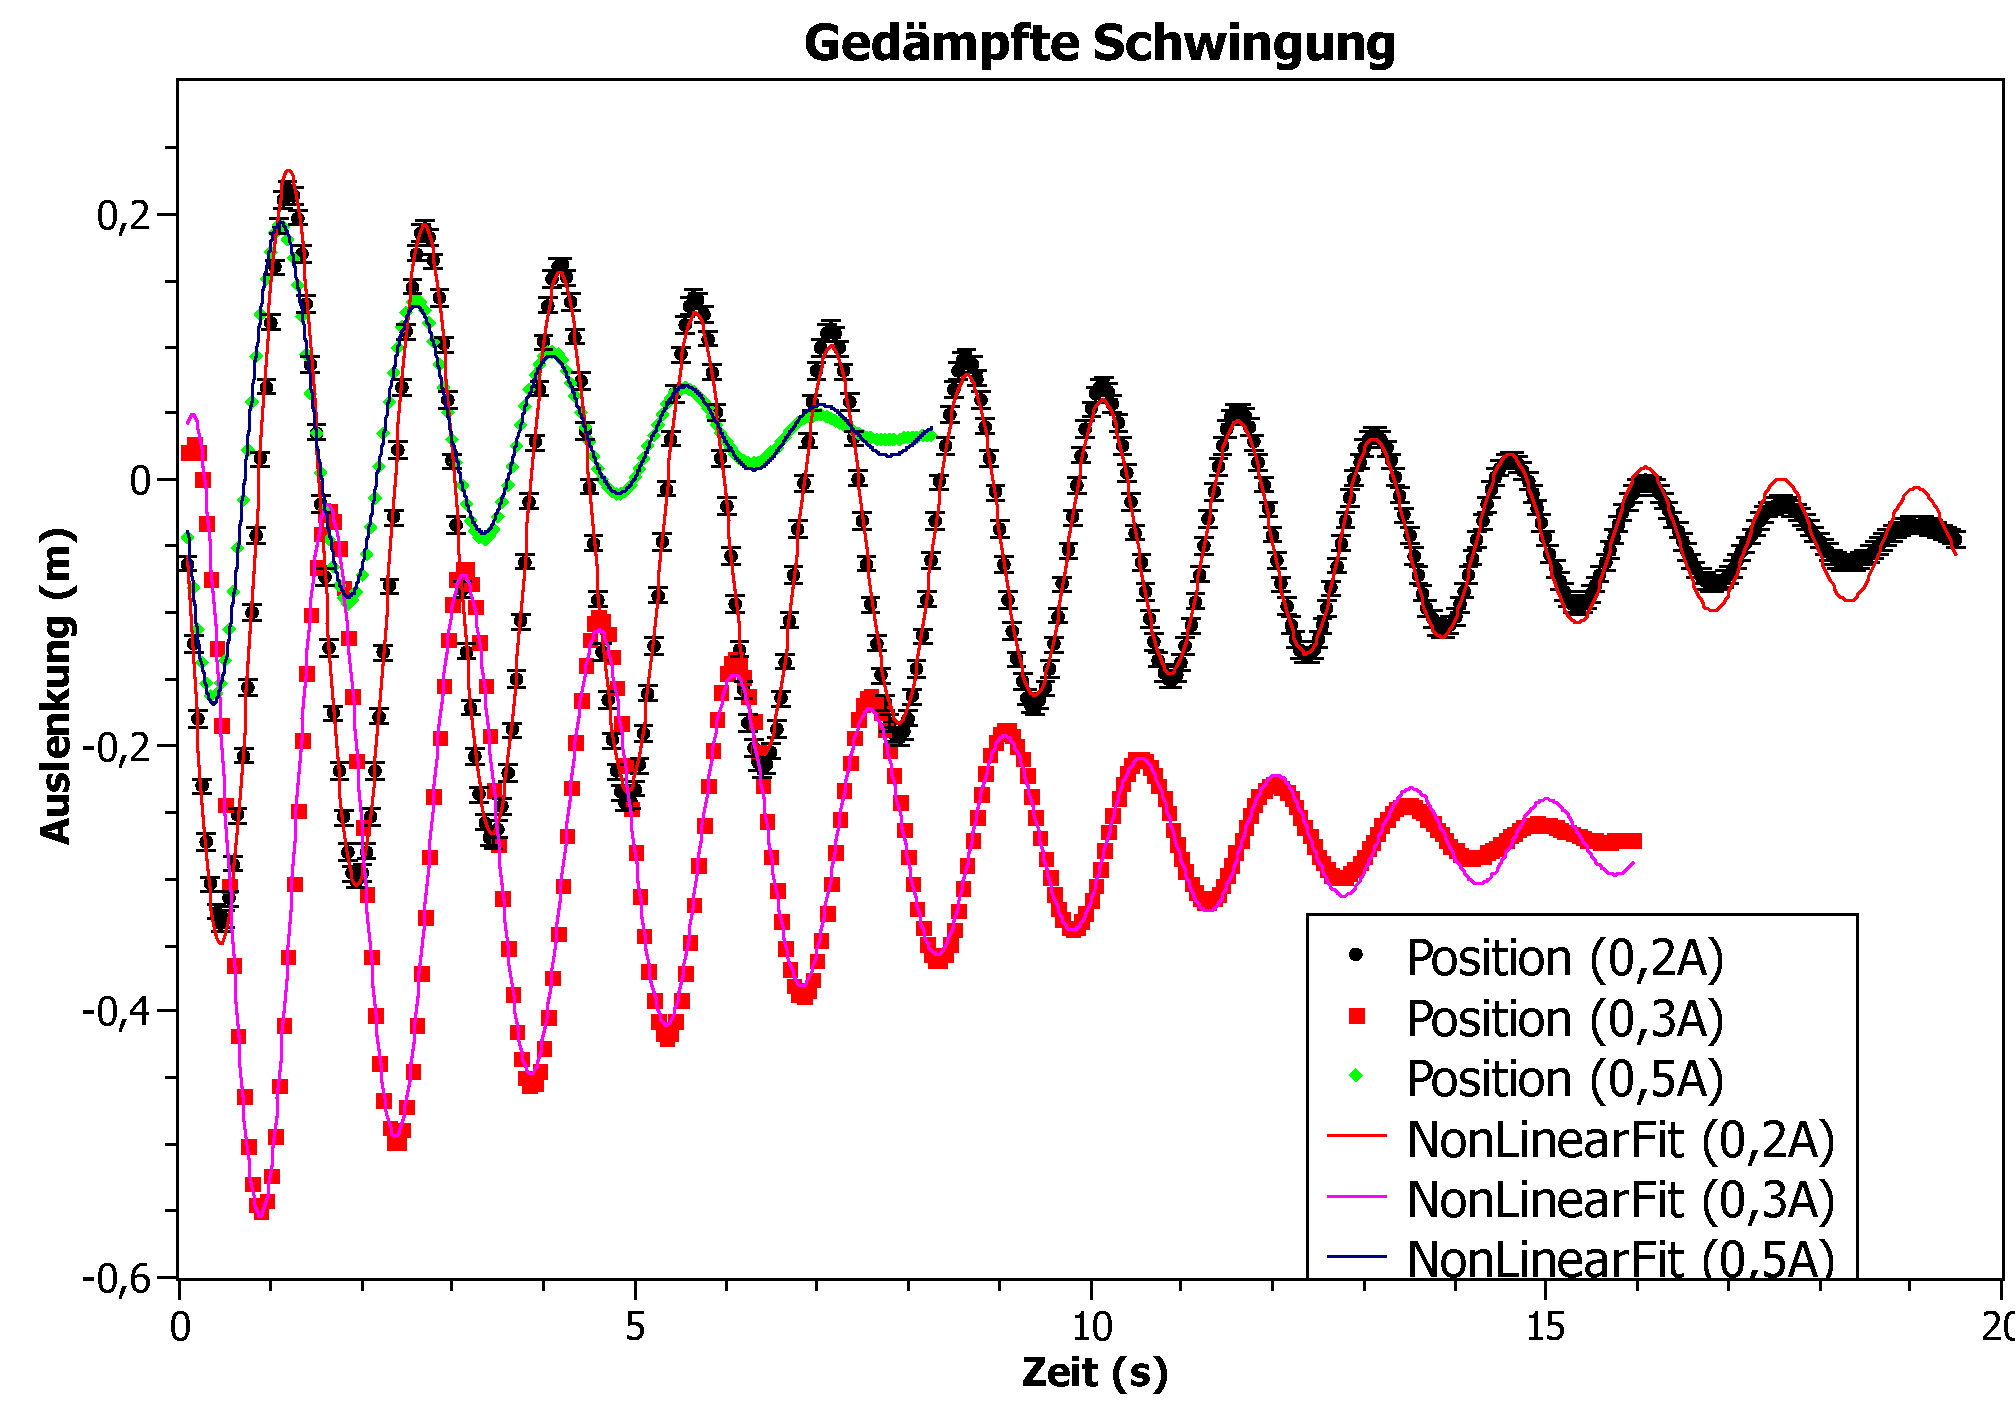
\includegraphics[width=1\textwidth]{Gedaempfte_Schwingung_Graph}
		\centering
		\caption{Das Ergebnis der mit dem Computer aufgezeichneten Messkurve für die gedämpfte Schwingung bei Betrieb der Wirbelstrombremse mit \SI{0,2}{\ampere}, \SI{0,3}{\ampere} und \SI{0,5}{\ampere}.}
		\label{gedämpfte_Schwingung}
		\centering
	\end{figure}
	Eine Anwendung desselben Fits auf die Messungen mit einer Wirbelstrombremse, durch die ein Strom $ I $ fließt, liefert folgendes Ergebnis in \cref{gedaempftTab} für die Frequenz $ f $ und die Dämpfung $ d $.\\
	\begin{table}[htb]
		\centering
		\begin{tabular}{ r | c | c | c |}
			$I /\si{\ampere}$& 0,2 & 0,3 & 0,5\\ \hline
			$f  /\si{\per \second}$ & \num{0,6717 \pm 0,0001} & \num{0,6728 \pm 0,0002} & \num{0,6741 \pm 0,0008}\\
			$d /\si{\per \meter}  $ & \num{0,108 \pm 0,001} & \num{0,159 \pm 0,001} & \num{0,337 \pm 0,005}
		\end{tabular}
		\caption{Ergebnisse des Fits für die Frequenz $ f $ und die Dämpfung $ d $ bei unterschiedlichen Stromstärken der Wirbelstrombremse}
		\label{gedaempftTab}
	\end{table}
	
	\subsection{Drehpendel mit Exzenter und Dämpfung}
	
	Um zunächst die Kalibrierkurve für den Zusammenhang zwischen Spannung am Tacho-Ausgang des Motors und Anregungsfrequenz aufzustellen, wurde ein Fit gemäß dem \enquote{Scaled Levenberg-Marquardt algorithm} mit der zugrunde liegenden Funktion
	\begin{equation}
	y(t) = a \sin ((x-b)2 \pi f) + c
	\end{equation}
	für jede der angelegten Spannungen durchgeführt. Aus diesen Fits ergeben sich Fehler, die alle kleiner sind als $ u_x = 0,002 $. Dann wurden in \cref{Kalibirierkurve} die Frequenzen gegen die Spannung aufgetragen. Die Unsicherheit des Multimeters, mit dem die Spannung gemessen wurde, wird im Folgenden betrachtet: \\
	Der Hersteller des Multimeters gibt eine Messtoleranz von ±0,5\% des abgelesenen Wertes für Gleichspannungsmessungen in den Messbereichen 2 V und 20 V an. Dies ist eine Typ B Unsicherheit mit rechteckiger WDF. Außerdem lässt sich die Spannung nur bis auf zwei Nachkommastellen ablesen, wodurch eine zusätzliche Ungenauigkeit von $\pm 0,005\si{V}$ entsteht. Dies ist ebenfalls eine Typ B Unsicherheit mit rechteckiger WDF. Insgesamt ergibt sich: \\
	$u_1= \frac{0,01}{2\sqrt{3}} \si{V} \approx 0,0029 \si{V}$ \\
	$u_2= \frac{2 \cdot 0,005 \cdot \text{Messwert}}{2 \sqrt{3}}$ \\ %kp ob das schön ist
	Für Messwerte kleiner \SI{20}{\volt} schätzen wir die Unsicherheit nach oben ab mit:
	\begin{equation*}
		\sqrt{(\frac{0,01 \cdot \text{Messwert}}{2 \sqrt{3}})^2 + 0,0029^2} \si{V} <  \SI{0,06}{\volt}
	\end{equation*}
	
	\begin{figure}[htb]
		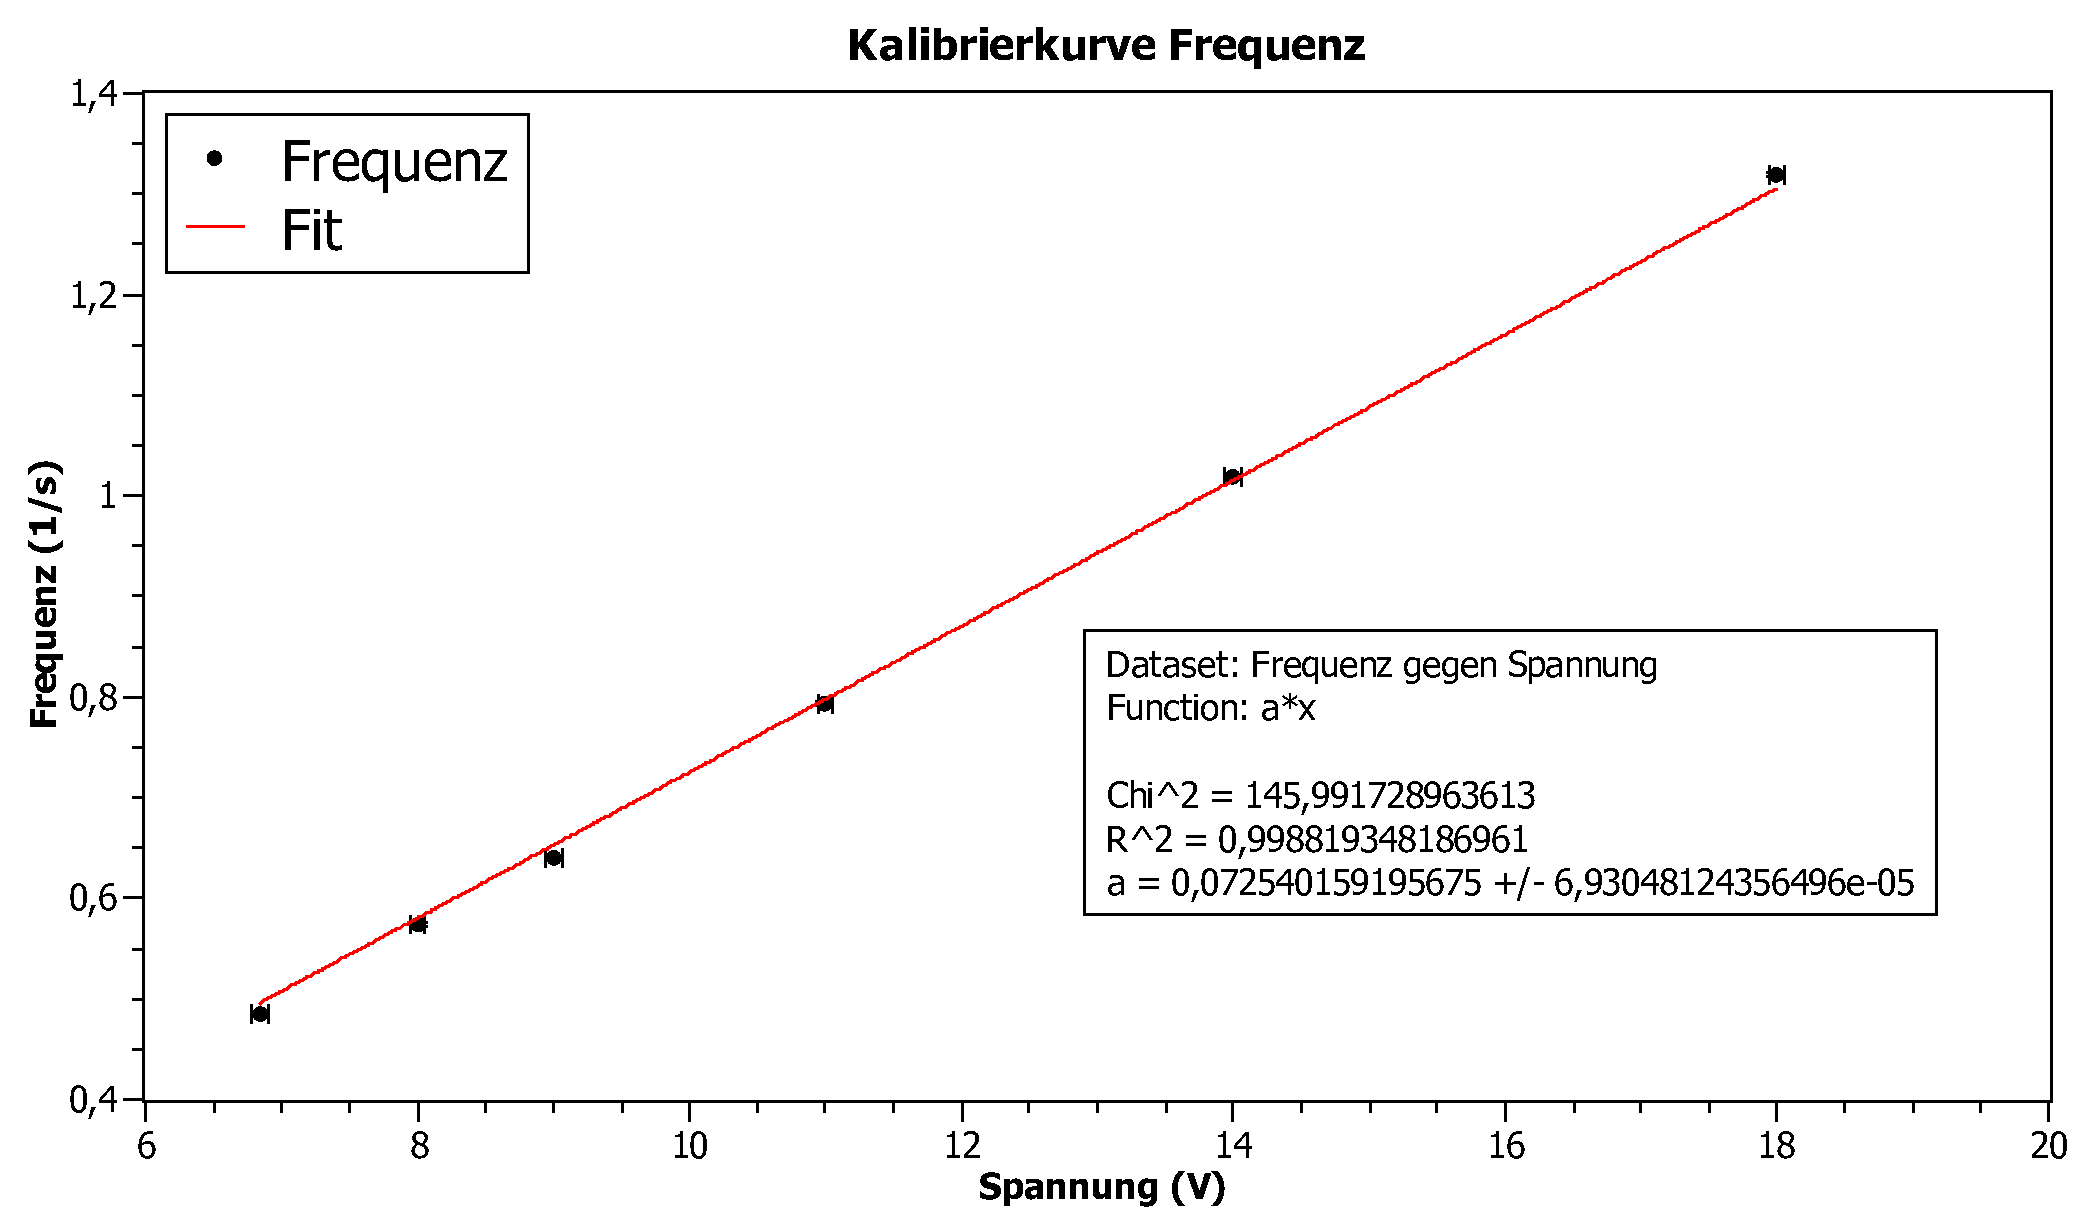
\includegraphics[width=1\textwidth]{Kalibrierkurve_Graph}
		\centering
		\caption{Hier ist die Abhängigkeit zwischen Spannung und Anregungsfrequenz dargestellt.}
		\label{Kalibirierkurve}
		\centering
	\end{figure}
	Aus \cref{Kalibirierkurve} lässt sich ein linearer Zusammenhang zwischen Spannung und Frequenz erkennen, der durch den Punkt (0,0) laufen muss, da der Motor ohne Spannung sich nicht bewegen kann. Wenn man einen dementsprechenden Fit durchführt, ergibt sich ein Zusammenhang von $ f_0 = U \cdot \SI{0,073 \pm 0,001}{\per \second \per \volt} $.
	
	
	\section{Schlussfolgerung}
	
	%\printbibliography
\end{document}
